\chapter{Simulation Models}  \label{sec:models}

\section{Parallel HOLD (PHOLD)} \label{sec:pholdModel}
The experimental analysis have been conducted using a parallelized version of the classic Hold synthetic benchmark called PHOLD. It has been used by many investigators because it has shown to effectively emulate the steady-state phase of a typical simulation~\cite{franceschini-15,tang-05}. Our PHOLD
implementation developed using MUSE provides several parameters
(specified as command-line arguments) summarized in Table ~\ref{tab:phold-params}. The benchmark consists of a 2-dimensional grid of LPs specified via the \textbf{rows} and \textbf{cols} parameters. The LPs are evenly partitioned across the MPI-processes used for simulation. The \textbf{imbalance} parameter influences the partition, with larger values skewing the partition as shown in Figure\ref{fig:phold}(a). The \textbf{imbalance} parameter has no impact in sequential simulations.


\begin{table}[!ht]\centering
\textbf{\caption{Parameters in PHOLD benchmark}}\label{tab:phold-params}
\begin{tabular}{lp{2.2in}}
\toprule
Parameter & Description \\
\midrule

\textbf{rows} & Total number of rows in model. \\

\textbf{cols} & Total number of columns in model. \#LPs = \textbf{rows}

\texttimes\/ \textbf{cols} \\

\textbf{eventsPerLP} & Initial number of events per LP. \\

\textbf{delay} or $\lambda$ & Value used with distribution -- Lambda
($\lambda$) value for exponential distribution \textit{i.e.,}
$P(x|\lambda)=\lambda e^{-\lambda x}$. \\

\textbf{\%selfEvents} & Fraction of events LPs send to self \\

\textbf{granularity} & Additional compute load per event. \\

\textbf{imbalance} & Fractional imbalance in partition to have more LPs on a MPI-process. \\

\textbf{simEndTime} & GVT when simulation logically ends.\\

\bottomrule
\end{tabular}
\end{table}

\begin{figure*}[ht]
\begin{minipage}{0.32\linewidth}
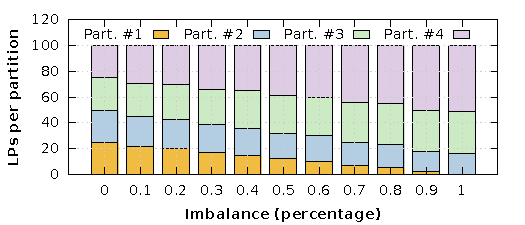
\includegraphics[width=\linewidth]{images/skew_data}
\centerline{(a) Impact of \textbf{imbalance}}
\end{minipage} 
\begin{minipage}{0.32\linewidth}
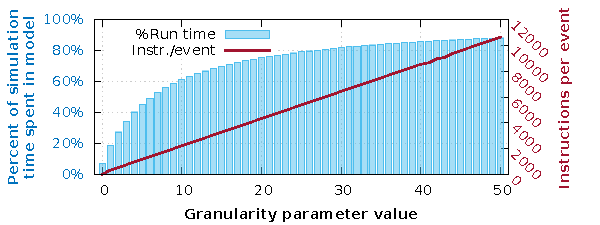
\includegraphics[width=\linewidth]{images/gran_info}
\centerline{(b) Impact of \textbf{granularity}}
\end{minipage} 
\begin{minipage}{0.32\linewidth}
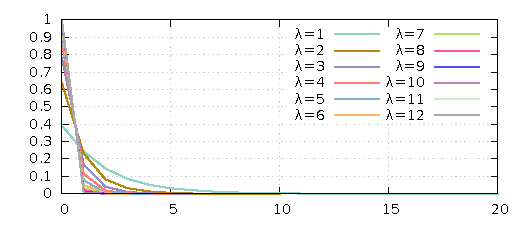
\includegraphics[width=\linewidth]{images/exp_delay_chart}
\centerline{(c) Impact of \textbf{delay} ($\lambda$)}
\end{minipage}
\textbf{\caption{Impact of varying key parameter values in the PHOLD model}}\label{fig:phold}
\end{figure*}
The PHOLD simulation commences with a fixed number of events for each LP, specified by the \textbf{eventsPerLP} parameter. For each event received by an LP a fixed number of trigonometric operations determined by \textbf{granularity} are performed to place CPU load. The impact of increasing the \textbf{granularity} parameter (no unit) is summarized in Figure 2(b) -- smaller values result in finer grained simulations. For each event, an LP schedules another event to a randomly chosen adjacent LP.  The \textbf{selfEvents} parameter controls the fraction of events that an LP schedules to itself.
The event timestamps are determined by a given \textbf{delay\--distrib} and \textbf{delay} or $\lambda$ parameters. Our experiments use an exponential distribution for timestamps, because it has shown to reflect event distribution commonly found in a broad range of simulation models~\cite{tang-05}. Time stamp of events is computed as $t_{recv}$ = LVT + 1 + $\lambda e^{-\lambda x}$. The impact of changing the $\lambda$ (\textit{i.e.,} \textbf{delay}) is shown in Figure \ref{fig:phold}(c) --smaller values of $\lambda$ provide a broader range of time stamp value for future events resulting in fewer concurrent events per LVT. Conversely, larger $\lambda$ values cause timestamps to be close to the current epoch, increasing both the number of concurrent events per LVT and the possibility of rollbacks. The impact of these parameters on scheduler queue performance were explored using 2,500 different configurations.


\begin{table}[!ht]\centering
\textbf{\caption{Parameters in PCS Model}} \label{tab:pcs-params}
\begin{tabular}{lp{2.2in}}
\toprule
Parameter & Description \\
\midrule

\textbf{rows} & Total number of rows in model. \\

\textbf{cols} & Total number of columns in model. \#Cells/LPs = \textbf{rows}

\texttimes\/ \textbf{cols}. \\

\textbf{portables} & The Portable represents a mobile phone unit that resides within the Cell for a period of time and then moves to one of the four neighboring Cells \\

\textbf{moveIntervalMean} &  This value represents the mean used for an exponential random distribution used to
generate the time when a portable will move to an adjacent cell. \\

\textbf{callIntervalMean} & The mean time between two successive calls to a portable associated with this Cell.  This value is the mean of an exponential random distribution from where the next call timestamp value is determined. \\

\textbf{callDurationMean} &  The mean call completion time. This value represents the mean used for a Poisson distribution used to generate the length/duration of a call to a portable. \\

\textbf{\#channels} & The maximum number of channels assigned to each PCS cell.\\

\textbf{imbalance} & Fractional imbalance in partition to have more LPs on a MPI-process. \\

\textbf{simEndTime} & GVT when simulation logically ends.\\

\bottomrule
\end{tabular}
\end{table}


\section{Personal Communication Service Network (PCS)}\label{sec:pcs}

The experimental analysis was also performed using a network communication simulation model named PCS. The model was developed to simulate large scale wireless communication networks~\cite{carothers-94}. The implementation uses parameters summarized in Table~\ref{tab:pcs-params}. The PCS model consists of cells (i.e. cellular towers) that transmit and receive phone calls made by mobile cellular phone units that reside at each Cell. A Cell is the central entity (LP) object type for the simulation. The Cells contain a fixed number of channels that are licensed to individual mobile phone units known as \textbf{Portables}. A \textbf{channel} is a wireless channel via which a \textbf{portable} can send/receive information from a Cell. A Portable at a given cell communicates to local or remote Portables, if a channel is available. Otherwise, the call is considered a blocked phone call. The Portables are mobile and travel to various cells throughout the network. The MUSE implementation of PCS models each cell as an LP and a portable as an event.

The PCS simulation commences with a fixed number of portables/events and channels for each Cell/LP, specified by the \textbf{portables} and \textbf{channels} parameters. The portables contain three exponentially distributed timestamps fields with means specified by \textbf{moveIntervalMean}, \textbf{callIntervalMean} and \textbf{callDurationMean} parameters. The minimum of the timestamps is used to determine the behavior of the portables (i.e., completion of a phone call, arrival of the next portable call at a cell, and the departure of a portable from its current cell to a neighboring cell). The PCS simulation will be used to validate resulting experimental analysis using the synthetic benchmark PHOLD.  The evaluation of the data structures using \textbf{PCS} provides a way to evaluate the persistence of trends and outcomes observed in the \textbf{PHOLD} simulation across a different model.   
